\section{Paper I: Deep residual networks for automatic sleep stage classification of raw polysomnographic waveforms}\label{sec:paperi}
\sectionmark{Olesen, Jennum, Peppard, Sorensen, \& Mignot, 2018}

% \begin{tcolorbox}[colframe=dtu-red!50, colback=white]
\begin{tcolorbox}[colframe=white]
\paragraph{Abstract} We have developed an automatic sleep stage classification algorithm based on deep residual neural networks and raw polysomnogram signals. 
Briefly, the raw data is passed through 50 convolutional layers before subsequent classification into one of five sleep stages. 
Three model configurations were trained on 1850 polysomnogram recordings and subsequently tested on 230 independent recordings. 
Our best performing model yielded an accuracy of 84.1\% and a Cohen's kappa of 0.746, improving on previous reported results by other groups also using only raw polysomnogram data. 
Most errors were made on non-REM stage 1 and 3 decisions, errors likely resulting from the definition of these stages. 
Further testing on independent cohorts is needed to verify performance for clinical use.
\end{tcolorbox}

\subsection{Methods}
\subsubsection{Data}
A database containing 2310 recordings extracted from the \ac{WSC} was used in this study.
Specific acquisition details concerning the \acp{PSG} are described in~\cite{Young1993,Young2008}.
The entire set of \ac{PSG} studies was randomly split into training (train), validation (eval), and testing (test) subgroups in an 8:1:1 ratio.
Detailed demographic information as well as relevant \ac{PSG} variables for all three subgroups are provided in~\cref{tab:sleep-stages:wsc_demographics} including \ac{AHI} and time spent in each sleep stage based on manual scoring. %No statistically significant differences between subgroups were found except for the amount of N1 and N2 sleep.

\subsubsection{Data processing pipeline}
Central and occipital \ac{EEG} from the right hemisphere, left and right \ac{EOG}, and chin \ac{EMG} channels were extracted from each \ac{PSG} study. 
To accommodate different equipment setups used for recording studies, each channel was upsampled to \SI{200}{\hertz}. %from either 100 Hz or 128 Hz to \SI{200}{\hertz}. %Ideally, this procedure will neither destroy nor add any information in the signals. 
Following resampling, signals were filtered using zero-phase Butterworth filters with frequency ranges recommended by the \ac{AASM}2016~\cite{Berry2016}. %, see~\cref{tab:aasm_filter}. 
Since dynamic ranges vary considerably across channels, each signal was soft-normalized using the \nth{5} and \nth{95} quantiles, such that 
\begin{equation}
    \mathbf{x}_{\mathrm{norm}} = 2~\frac{\mathbf{x} - \mathrm{Q}_{0.05}(\mathbf{x})}{\mathrm{Q}_{0.95}(\mathbf{x}) - \mathrm{Q}_{0.05}(\mathbf{x})} - 1,
\end{equation}
where $\mathbf{x}_{\mathrm{norm}}$ denotes the normalized version of the signal $\mathbf{x}$, and $\mathrm{Q}_{0.05}(\mathbf{x})$ and $\mathrm{Q}_{0.95}(\mathbf{x})$ denotes the \nth{5} and \nth{95} percentile, respectively.
Doubling and subtracting by one rescales $\mathrm{Q}_{0.05}(\mathbf{x})$ and $\mathrm{Q}_{0.95}(\mathbf{x})$ to $-1$ and $1$, respectively.

Finally, each signal was segmented into \SI{30}{\second} epochs corresponding to \ac{AASM}2016 criteria~\cite{Berry2016}, resulting in a tensor $\mathbf{X}$\graffito{We introduce a singleton dimension, as the {\texttt{tf.layers.conv1d}} implementation in TensorFlow reshapes the input argument to match \texttt{tf.layers.conv2d}.} with elements 
\begin{equation}
    (x_{n,c,\cdot,t}) \in \real{N\times C\times 1 \times T},
\end{equation}
with $N=16$, $C=5$, and $T=6000$ being batch size, number of signals, and number of timesteps for one epoch, respectively. %is the batch size, $C=5$ designates the signal channels, and $T=6000$ designates samples in the \SI{30}{\second} epoch at a sampling rate of \SI{200}{\hertz}.

\begin{table}
\centering
\small
\begin{threeparttable}
    % \footnotesize
    \caption[\acs{WSC} subset demographics]{\acs{WSC} demographics for each subgroup.}
    \label{tab:sleep-stages:wsc_demographics}
    \begin{tabular}{@{}lcccc@{}}
        \toprule
                                                & \textbf{Train}             & \textbf{Eval}              & \textbf{Test}              & \textbf{\textit{p}-value} \\ \midrule
        \textit{n} (male)                       & 1850 (1010)       & 230 (112)         & 230 (120)         & 0.210             \\
        Age, years                             & $ 59.2 \pm 8.4 $  & $ 59.9 \pm 8.5 $  & $ 60.4 \pm 8.2 $  & 0.092             \\
        \acs{BMI}, \si{\kilo\gram\per\metre\squared} & $ 31.7 \pm 7.2 $  & $ 31.0 \pm 6.9 $  & $ 32.2 \pm 7.7 $  & 0.203             \\
        \acs{AHI}, \si{\per\hour}                    & $ 12.6 \pm 15.6 $ & $ 11.5 \pm 14.9 $ & $ 12.4 \pm 16.2 $ & 0.600            \\ \midrule
        \acs{TST}, \si{\hour}                & $ 7.4 \pm 0.8 $   & $ 7.4 \pm 0.7 $   & $ 7.4 \pm 0.8 $   & 0.947            \\ 
        \acs{W}, \%                                & $ 18.5 \pm 11.3 $ & $ 17.2 \pm 11.1 $ & $ 19.6 \pm 11.8 $ & 0.071             \\
        \acs{N1}, \%                                 & $ 8.2 \pm 4.5 $   & $ 8.8 \pm 5.6 $   & $ 8.9 \pm 5.1 $   & $\mathbf{0.038}$  \\
        \acs{N2}, \%                                 & $ 54.2 \pm 10.3 $ & $ 54.0 \pm 10.9 $ & $ 52.4 \pm 11.0 $ & $\mathbf{0.048}$  \\
        \acs{N3}, \%                                 & $ 5.8 \pm 6.4 $   & $ 6.4 \pm 7.0 $   & $ 6.0 \pm 7.0 $   & 0.433             \\
        \acs{REM}, \%                                & $ 13.3 \pm 5.9 $  & $ 13.7 \pm 5.8 $  & $ 13.2 \pm 5.7 $  & 0.635             \\ \bottomrule
    \end{tabular}
    \begin{tablenotes}
        \small
        \item Values are shown as mean \(\pm\) standard deviation across subjects. Significant \textit{p}-values highlighting differences between subsets are highlighted in bold as tested with \(\chi^2\) test (population proportions) and \acs{ANOVA} (rest). %
        \describe{WSC}; %
        \describe{BMI}; %
        \describe{AHI}; %
        \describe{TST}; %
        \describe{W}; %
        \describe{N1}; %
        \describe{N2}; %
        \describe{N3}; %
        \describe{REM}.
    \end{tablenotes}
\end{threeparttable}
\end{table} 

\subsubsection{Deep residual network model}
We applied a deep learning model inspired by the residual network models proposed in~\cite{He2016,He2016b}.
These types of models employ residual skip connections between layers in order to maintain a proper gradient backpropagation\graffito{This is also known as the vanishing gradient problem and is especially problematic in very deep networks and \acsp{RNN}.} through the network.
This feature allows for extremely deep network structures, and a specific variant of this model with 152 layers came in \nth{1} place in the ILSVRC '15 image classification competition~\cite{He2016}.

\paragraph{Network architecture}
\begin{figure}[t]
    \begin{adjustwidth*}{}{-\marginparwidth-\marginparsep}
    \centering
    % 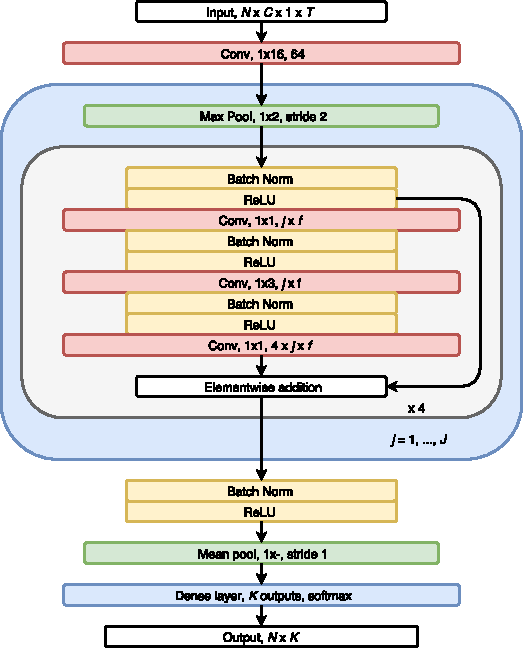
\includegraphics[height=0.5\textheight]{figures/ResNet_EMBC_compressed.pdf}
    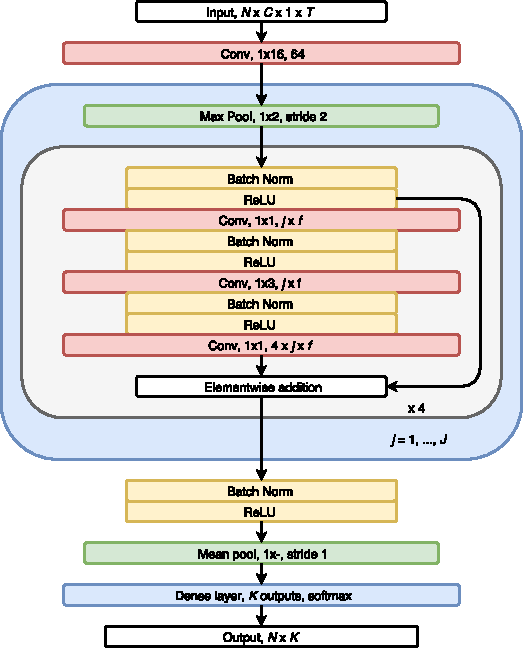
\includegraphics[width=0.9\textwidth]{figures/ResNet_EMBC_compressed.pdf}
    \caption[\acs{MASSC} network architecture]{\ac{MASSC} network architecture. The input tensor containing \ac{EEG}, \ac{EOG}, and \ac{EMG} has shape $(N, C, 1, T)$, where $N$, $C=5$, $T=6000$ correspond to the batch size, number of signals, and length of each \SI{30}{\second} epoch, respectively. The output tensor has shape $N\times K$ with $K=5$ sleep stages, while $L=4$, and $f=16$ is the number of block layers and base number of filters.}
    \label{fig:sleep-stages:network}
    \end{adjustwidth*}
\end{figure}
The residual network model is illustrated in~\cref{fig:sleep-stages:network}. 
Briefly, the bulk network comprised 50 convolutional (conv) and dense layers arranged in four block layers of four bottlenecked residual blocks each. 

A single bottleneck residual block contains three triplets of a batch normalization layer, a \ac{ReLU} activation layer, and a conv layer. 
This pre-activation configuration has shown benefits with regards to trainability and generalization compared to vanilla residual blocks~\cite{He2016b}.
Projection shortcuts were used between the first \ac{ReLU} and conv layers to the output of the last conv layer.
Kernel sizes were set to $1\times1$ for the first and third conv layers, and $1\times3$ for the second conv layer.
The number of output filters for each residual block was $l\times f$ with $l$ being the block layer index and $f=16$, resulting in a total of 256 filters after the final conv layer.

Prior to the bottleneck blocks, the input tensor $\mathbf{X}$ was passed through an initial conv layer consisting of 64 $1\times16$ filters, and then through a maximum pooling (max pool) layer with a $1\times2$ kernel and stride size, effectively reducing the time-resolution by a factor of 2.
This max pool operation was implemented in the beginning of each block layer.

The output tensor from the block layers was subsequently passed to a final batch normalization and \ac{ReLU} activation layer, followed by a mean pooling layer to reduce the tensor to $\mathbf{X} = \left(x_{nk}\right) \in \real{N\times 256}$.
Finally, a fully connected layer with $K=5$ output units corresponding to the sleep stages resulted in the following output tensor
\begin{equation}
    \mathbf{P} = \left(p_{nk}\right) \in \real{N \times K}, \quad p_{nk} = \frac{\exp{(z_{nk})}}{\sum_{k}^{K} \exp{(z_{nk})}}
\end{equation}
with $p_{nk}$ containing the softmax activations of the output units $z_{nk}$ from the fully connected layer for the $n$th subject and the $k$th sleep stage.
The predicted class for the $n$th subject can then be calculated as
\begin{equation}\label{eq:argmax}
    \hat{y}_n = \argmax_{k} p_{nk}.
\end{equation}

\paragraph{Training setup}
The optimization problem was constructed using cross entropy loss across $K$ classes and $N$ epochs as objective function, such that
\begin{equation}
    \mathcal{L}(\mathbf{p}_{n} |\, \mathbf{y}_{n},\boldsymbol{\theta}_w) = -\sum_{k=1}^{K}{y_{nk}\log{p_{nk}}},
\end{equation}
is the calculated cross entropy loss for epoch $n$ given predicted class probabilities $\mathbf{p}_n$, true class labels $\mathbf{y}_n$, and the set of current weights $\boldsymbol{\theta}_w$.
Then, the average cost across a batch of data is
\begin{equation}
    \mathcal{C}(\mathbf{P} |\, \mathbf{Y},\boldsymbol{\theta}_w) = \frac{1}{N}\sum_{n=1}^{N}{\mathcal{L}(\mathbf{p}_{n} | \mathbf{y}_{n},\boldsymbol{\theta}_w)}\label{eq:cost}.
\end{equation}
The cost function was optimized using the Adam optimization algorithm with default hyperparameters~\cite{Kingma2015}.
Weights were initialized using variance scaling~\cite{He2015a}, and we applied weight decay during training with a decay factor of $\lambda=10^{-4}$.
The initial learning rate was set to $\alpha=10^{-3}$ and was multiplied by $0.1$ every \num{50000} steps.

In order to investigate the effect of the imbalanced data on the network performance, we trained the following three different configurations.
First, we defined a \textit{baseline} configuration as described in the previous sections.
The second was a \textit{weighted} configuration, where the cost function in~\cref{eq:cost} was replaced with an average weighted by the inverse frequency for the correct class, such that
\begin{equation}
    \mathcal{C}(\hat{\mathbf{Y}} |\, \mathbf{Y},\boldsymbol{\theta}_w) = \frac{\sum_{n}^{N} \omega_{n}(\mathbf{y}_{n}) \mathcal{L}(\hat{\mathbf{y}}_{n} | \mathbf{y}_{n},\boldsymbol{\theta}_w)}{\sum_{n}^{N} \omega_{n}(\mathbf{y}_{n})},
\end{equation}
where $\omega_{n}(\mathbf{y}_{n})$ is the inverse frequency for the correct class for the $n$th subject in the current batch.
Finally, a \textit{balanced} configuration was tested, in which we performed resampling of the training dataset in order to balance classes.
We oversampled the \ac{N1}, \ac{N3}, and \ac{REM} classes with replacement, while undersampling the \ac{N2} class in order to have approximately equal fractions of each class in total.

% Models were implemented in TensorFlow 1.4~\cite{Abadi2016}, and trained on a single workstation running Ubuntu 16.04 with a Ryzen 7 1700X 8-core CPU, an NVIDIA GTX 1080 Ti GPU with 11 GB memory, and 32 GB RAM memory.

\subsubsection{Performance metrics}
Individual precision, recall and F1 scores (Pr, Re, F1) were calculated for each sleep stage and subsequently aggregated for each recording by stage frequency weighting, such that
\begin{equation}
    \mathrm{Pr}_{nk} = \frac{\mathrm{TP}}{\mathrm{TP} + \mathrm{FP}}, \quad \mathrm{Pr}_{n} = \frac{\sum_{k}{\beta_{nk} \mathrm{Pr}_{nk}}}{\sum_{k}\beta_{nk}}
\end{equation}
\begin{equation}
    \mathrm{Re}_{nk} = \frac{\mathrm{TP}}{\mathrm{TP} + \mathrm{FN}}, \quad \mathrm{Re}_{n} = \frac{\sum_{k}{\beta_{nk} \mathrm{Re}_{nk}}}{\sum_{k}\beta_{nk}}
\end{equation}
\begin{equation}
    \mathrm{F1}_{nk} = 2 \cdot \frac{\mathrm{Pr}_{nk} \cdot \mathrm{Re}_{nk}}{\mathrm{Pr}_{nk} + \mathrm{Re}_{nk}}, \quad \mathrm{F1}_{n} = \frac{\sum_{k}{\beta_{nk} \mathrm{F1}_{nk}}}{\sum_{k}\beta_{nk}},
\end{equation}
where $\beta_{nk}$ is the frequency of stage $k$ for recording $n$, and TP, FP and FN are true positives, false positive, and false negatives, respectively. 
Overall accuracy (Acc) and Cohen's kappa ($\kappa$) were also calculated for each recording.
All metrics were summarized by mean and standard deviations.

\subsubsection{Statistical tests}
Demographic and \ac{PSG} variables were tested with \acp{ANOVA} after establishing normality, while gender was tested with a $\chi^{2}$ test.
Significance was set at $\alpha=0.05$.

\subsection{Results and discussion}
Performance metrics for the train and eval subgroups are shown in~\cref{tab:sleep-stages:train_eval_performance}.
Not accounting for Pr, the baseline configuration compares favorably to the weighted and balanced configurations on both subgroups with an average accuracy of \SI{85.0}{\percent} and a Cohen's kappa of \SI{75.4} on the eval subgroup.
Since the training data is imbalanced in favor of \ac{N2}, it would be fair to assume overfitting to the majority class.
However, the lower spread in both precision and recall does not support this.

\begin{figure}[tb]
\begin{adjustwidth*}{}{-\marginparwidth-\marginparsep}
    \centering
    % 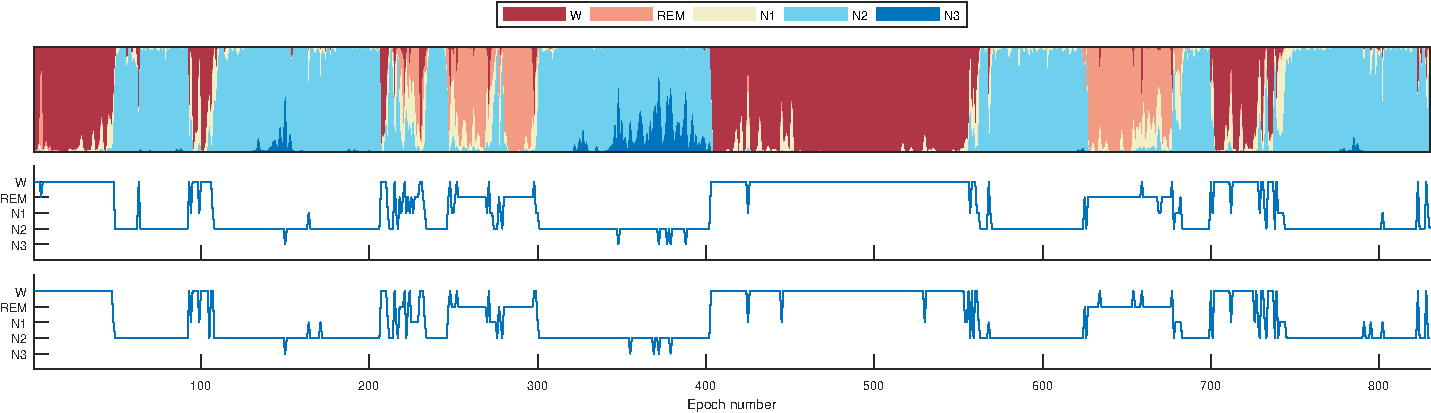
\includegraphics[width=\linewidth]{figures/test_maxacc_id1627-eps-converted-to.pdf}
    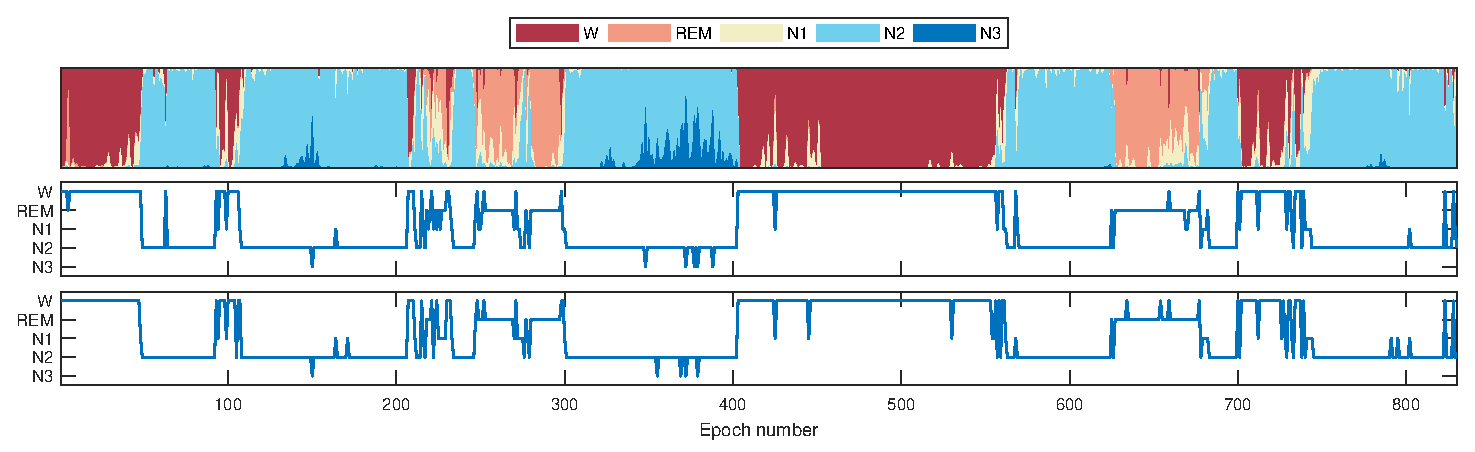
\includegraphics[width=\linewidth]{figures/paper-i/test_maxacc_id1627.eps}
    \caption[\acs{MASSC} hypnodensity example]{Top: hypnodensity graph of per-epoch probability distributions, middle: automatically scored hypnogram by applying~\cref{eq:argmax}. Bottom: manually scored hypnogram. Note the intrusions of \ac{N3} into \ac{N2} around epoch 150 and 370, and \ac{N1} into \ac{W} around 420.}
    \label{fig:slee-stages:hypnodensity}
\end{adjustwidth*}
\end{figure}

\begin{table}
    \small
    % increase table row spacing, adjust to taste
    % \renewcommand{\arraystretch}{1.3}
    \centering
    \begin{threeparttable}
    \caption[\acs{MASSC} train and validation performance, \acs{WSC}]{Averaged performance metrics for configurations.}% across train and eval subgroups.}
    \label{tab:sleep-stages:train_eval_performance}
    \begin{tabular}{@{}clccc@{}}
        \toprule
                              &          & \textbf{Baseline}          & \textbf{Weighted}          & \textbf{Balanced}          \\ \midrule
        \multirow{5}{*}{\textbf{Train}} & Acc, \%      & $ \mathbf{86.1 \pm 5.5} $ & $ 79.4 \pm 7.1 $ & $ 80.4 \pm 7.3 $ \\
                              & $\kappa$, \% & $ \mathbf{77.1 \pm 8.6} $ & $ 69.5 \pm 9.7 $ & $ 70.7 \pm 9.8 $ \\
                              & Pr, \%       & $ 87.1 \pm 4.9 $ & $ 88.7 \pm 4.1 $ & $ \mathbf{88.9 \pm 4.0} $ \\
                              & Re, \%       & $ \mathbf{86.1 \pm 5.5} $ & $ 79.4 \pm 7.1 $ & $ 80.4 \pm 7.3 $ \\
                              & F1, \%       & $ \mathbf{85.3 \pm 6.1} $ & $ 81.8 \pm 6.6 $ & $ 82.6 \pm 6.9 $ \\ \midrule
        \multirow{5}{*}{\textbf{Eval}}  & Acc, \%      & $ \mathbf{85.0 \pm 6.1} $ & $ 78.4 \pm 7.3 $ & $ 79.7 \pm 7.4 $ \\
                              & $\kappa$, \% & $ \mathbf{75.4 \pm 9.5} $ & $ 68.1 \pm 10.5 $ & $ 69.7 \pm 10.0 $ \\
                              & Pr, \%       & $ 86.3 \pm 5.3 $ & $ 87.8 \pm 4.8 $ & $ \mathbf{88.0 \pm 4.9} $ \\
                              & Re, \%       & $ \mathbf{85.0 \pm 6.1} $ & $ 78.4 \pm 7.3 $ & $ 79.7 \pm 7.4 $ \\
                              & F1, \%       & $ \mathbf{84.0 \pm 7.2} $ & $ 80.7 \pm 7.1 $ & $ 81.9 \pm 7.1 $ \\ \bottomrule
    \end{tabular}
    \begin{tablenotes}
    \item Metrics are shown as mean \(\pm\) standard deviations across each \ac{PSG}. Best performing model for each metric is shown in bold.
    \end{tablenotes}
    \end{threeparttable}
\end{table}

\begin{table}[tb]
    \small
    % increase table row spacing, adjust to taste
    % \renewcommand{\arraystretch}{1.3}
    \setlength{\tabcolsep}{4pt}
    \caption[\acs{MASSC} test group confusion matrix, \acs{WSC}]{Aggregated confusion matrix and stage-specific performance metrics in test subgroup.}
    \label{tab:sleep-stages:test_performance_aggregated}
    \centering
    \begin{threeparttable}
    \begin{tabular}{@{}llcccccccc@{}}
        \toprule
         & & \multicolumn{5}{c}{\textbf{Automatic}} & & & \\ \cline{2-7}
                 & \acs{W}     & \acs{W}   & \acs{N2}    & \acs{N3}   & \acs{REM}   & Pr, \% & Re, \% & F1, \% \\ \midrule
        \multirow{5}{*}{\textbf{Manual}} & \acs{W}        & 37980 & 1322 & 852   & 2    & 327   & 84.3    & 93.8    & 88.8    \\
         & \acs{W}       & 3922  & 8784 & 3545  & 0    & 2193  & 51.9    & 47.6    & 49.7    \\
         & \acs{N2}       & 1756  & 5136 & 99564 & 1091 & 991   & 88.6    & 91.7    & 90.2    \\
         & \acs{N3}       & 18    & 1    & 7932  & 4063 & 14    & 78.8    & 33.8    & 47.3    \\
         & \acs{REM}        & 1361  & 1680 & 465   & 0    & 23931 & 87.2    & 87.2    & 87.2    \\ \bottomrule
    \end{tabular}
    \begin{tablenotes}
        \small
        \item%
        \describe{W}; %
        \describe{N1}; %
        \describe{N2}; %
        \describe{N3}; %
        \describe{REM}.
    \end{tablenotes}
    \end{threeparttable}
\end{table}


Evaluating the baseline model on the test subgroup, only a slight drop in accuracy and $\kappa$ is observed, indicating that the model generalizes well, see~\cref{tab:sleep-stages:test_performance_aggregated} and~\cref{tab:sleep-stages:test_performance_average}.
The lowest sensitivity is obtained for \ac{N1} and \ac{N3}, which is in accordance with clinical experience reported in the literature~\cite{Younes2017, Rosenberg2013, Norman2000, Younes2016}.
N1 is a transitional stage between wakefulness, drowsiness and sleep often containing beta and alpha activity in epochs of low interscorer agreement, which explains the low predictive power in the confusion matrix.
The sleep continuum is also apparent in~\cref{fig:slee-stages:hypnodensity} which shows the manually and automatically scored hypnograms in the middle and bottom traces, and the hypnodensity graph in the top trace for a representative subject in the test subgroup.
The hypnodensity is a probabilistic representation of the hypnogram, which has found use in the detection of narcolepsy and Parkinson's disease~\cite{Koch2014, Christensen2014, Stephansen2018}.

Our baseline model attains favorable performance when comparing to the results reported for the raw waveform CNN model in~\cite{Biswal2017} with both higher accuracy and Cohen's kappa.
However, it should be stressed that~\cite{Biswal2017} only used \ac{EEG} channels from 9000 recordings, while our model uses both \ac{EEG}, \ac{EOG} and \ac{EMG} data, but only from 1850 recordings.
Furthermore, our baseline model performs only slightly worse compared to the best-performing model in~\cite{Biswal2017} without using any memory networks.
This indicates a performance gain by adding recurrent networks, such as long short-term memory cells, to our network.

A possible limiting factor to our model is the filter kernels.
The small filter sizes in block layers might not be able to accurately capture the physiological dynamics, but there are indications that many, smaller kernels are preferable to fewer, larger kernels when comparing model complexity versus computational costs~\cite{Szegedy2015}.

Future work will include adding more data to balance classes, and adding long short-term memory cells to the network in order to model temporal dynamics between epochs.
\begin{table}[tb]
    \small
    \centering
    \begin{threeparttable}
    \caption[MASSCv1 overall test performance, \acs{WSC}]{Performance across recordings in test subgroup.}
    \label{tab:sleep-stages:test_performance_average}
    \begin{tabular}{@{}ccccc@{}}
    \toprule
        \textbf{Accuracy}              & $\boldsymbol{\kappa}$         & \textbf{Pr}               & \textbf{Re}               & \textbf{F1}               \\ \midrule
        $ 84.1 \pm 6.9 $ & $ 0.746 \pm 0.099 $ & $ 85.7 \pm 6.1 $ & $ 84.1 \pm 6.9 $ & $ 83.1 \pm 7.6 $ \\ \bottomrule
    \end{tabular}
    \begin{tablenotes}
    \item Values are shown as mean \(\pm\) standard deviation across \acs{PSG}. Pr: precision; Re: recall.
    \end{tablenotes}
    \end{threeparttable}
\end{table}
